\chapter{Spin, isospin, couleur et auto-interaction des gluons}

\section{La chromodynamique quantique par analogie avec l’électrodynamique}

La chromodynamique quantique est un sujet trop vaste pour être développé entièrement en un seul cours. Nous chercherons ici à en donner une représentation intuitive de base plutôt qu’à en exposer les mathématiques plus approfondies.

L’électrodynamique quantique est la théorie des électrons et des photons. C’est aussi la théorie quantique de la force de Coulomb. Si l’on traite le noyau d’un atome comme une source fixe de champ électrique, sans s’interroger sur son mouvement ni sur sa structure interne, l’électrodynamique quantique est la théorie de l’atome.

La chromodynamique quantique joue un rôle analogue pour les quarks et les gluons. Elle décrit les particules elles-mêmes, les forces qui s’exercent entre elles et les objets composites qu’elles forment. Ces objets composites sont appelés \emph{hadrons}. Les protons et les neutrons sont des baryons : ils portent un nombre net de quarks, ou, de manière équivalente, un nombre baryonique non nul. Les mésons sont des combinaisons de quark--antiquark. Les baryons comme les mésons contiennent également des gluons.

Les gluons sont électriquement neutres, mais ils fournissent le champ qui lie les quarks. À cet égard, le champ de gluons joue un rôle analogue à celui du champ électromagnétique qui lie les atomes.

Avant d’introduire la couleur et les gluons, il est utile de revenir aux mathématiques du spin. Les mêmes mathématiques réapparaissent presque directement dans l’\emph{isospin}, et un schéma apparenté se retrouve dans la théorie de la couleur. La théorie des groupes sous-tend ces constructions, mais on peut développer les notions nécessaires à partir du moment cinétique.

\section{Multiplets de moment cinétique}

Les composantes du moment cinétique vérifient
\begin{equation}
[L_x,L_y]=i\hbar L_z,
\end{equation}
ainsi que les relations cycliques correspondantes
\begin{equation}
[L_y,L_z]=i\hbar L_x,
\qquad
[L_z,L_x]=i\hbar L_y.
\end{equation}
Les trois composantes ne commutent pas ; elles ne peuvent donc pas toutes être mesurées simultanément. On choisit alors un axe, conventionnellement l’axe \(z\), et l’on étiquette les états par la composante du moment cinétique selon cet axe.

Ce choix ne brise pas la symétrie de rotation dans la nature. Il ne brise la symétrie que dans la description, en sélectionnant une direction pour tenir les comptes.

Les valeurs permises de la composante \(z\) sont quantifiées et diffèrent d’une unité de \(\hbar\). En posant \(\hbar=1\) pour énumérer ces valeurs, un multiplet de spin \(\ell\) contient
\begin{equation}
m=\ell,\ell-1,\ldots,-\ell.
\end{equation}
Le nombre d’états indépendants est donc
\begin{equation}
2\ell+1.
\end{equation}

Il est utile d’écrire explicitement les premiers multiplets :
\begin{align}
\ell=0:&\qquad m=0,\\
\ell=\frac12:&\qquad m=\frac12,-\frac12,\\
\ell=1:&\qquad m=1,0,-1,\\
\ell=\frac32:&\qquad
m=\frac32,\frac12,-\frac12,-\frac32,\\
\ell=2:&\qquad m=2,1,0,-1,-2.
\end{align}

Pour ce qui nous occupe, le spin demi-entier caractérise les fermions et le spin entier, les bosons. L’électron est une particule de spin \(\tfrac12\). Une particule de spin nul n’a aucun moment cinétique. Le photon a un spin égal à un, et des états de spin un se rencontrent également dans les atomes et les noyaux. Les atomes et les noyaux peuvent aussi avoir un spin \(\tfrac32\), et le même décompte se poursuit pour les spins supérieurs.

La notation doit distinguer le spin total de sa composante. Le nombre \(\ell\) désigne le multiplet et est aussi la valeur maximale possible de la composante \(z\). Le nombre \(m\) désigne un état particulier de ce multiplet. Ainsi, un objet de spin un possède trois états, tandis qu’un objet de spin \(\tfrac12\) en possède deux.

\section{Combinaison de deux particules de spin un demi}

Considérons deux particules de spin \(\tfrac12\) et négligeons leur moment cinétique orbital. Leur espace produit de spins contient quatre états de base :
\begin{equation}
|\uparrow\uparrow\rangle,\qquad
|\uparrow\downarrow\rangle,\qquad
|\downarrow\uparrow\rangle,\qquad
|\downarrow\downarrow\rangle.
\end{equation}
Les composantes correspondantes selon \(z\) sont
\begin{align}
|\uparrow\uparrow\rangle &: m=+1,\\
|\uparrow\downarrow\rangle &: m=0,\\
|\downarrow\uparrow\rangle &: m=0,\\
|\downarrow\downarrow\rangle &: m=-1.
\end{align}

L’état où les deux spins sont orientés vers le haut montre qu’un multiplet de spin un doit exister : la composante \(z\) maximale vaut \(+1\). Un multiplet de spin un ne comporte que trois états,
\begin{equation}
m=+1,\quad 0,\quad -1.
\end{equation}
Or, l’espace produit contient quatre états, dont deux états indépendants avec \(m=0\). Ils ne peuvent pas tous appartenir à un seul multiplet de spin un. L’état supplémentaire ne peut pas être de spin deux, car un multiplet de spin deux compterait cinq états. Les quatre états produits doivent donc se répartir en trois états de spin un et un état de spin nul.

Quelle combinaison des deux états de base \(m=0\) appartient au multiplet de spin un ? Échangeons les deux particules. Les états où les spins sont alignés restent inchangés :
\begin{equation}
|\uparrow\uparrow\rangle\longrightarrow|\uparrow\uparrow\rangle,
\qquad
|\downarrow\downarrow\rangle\longrightarrow|\downarrow\downarrow\rangle.
\end{equation}
En revanche, les états produits mixtes sont échangés :
\begin{equation}
|\uparrow\downarrow\rangle
\longleftrightarrow
|\downarrow\uparrow\rangle.
\end{equation}
Leur somme est symétrique sous cet échange :
\begin{equation}
|\uparrow\downarrow\rangle+|\downarrow\uparrow\rangle.
\end{equation}
La normalisation introduit un facteur \(1/\sqrt2\) :
\begin{equation}
|1,0\rangle
=
\frac{|\uparrow\downarrow\rangle
      +|\downarrow\uparrow\rangle}{\sqrt2}.
\end{equation}

\begin{figure}[h]
\centering
\includegraphics[width=0.78\textwidth]{lecture_02_figure_02.png}
\caption{Combinaison symétrique de spins mixtes formant le membre \(m=0\) du triplet de spin un.}
\lectureframe{00:15:08}
\end{figure}

Avec les deux états alignés, cela donne le triplet de spin un :
\begin{align}
|1,+1\rangle &=|\uparrow\uparrow\rangle,\\
|1,0\rangle &=
\frac{|\uparrow\downarrow\rangle
      +|\downarrow\uparrow\rangle}{\sqrt2},\\
|1,-1\rangle &=|\downarrow\downarrow\rangle.
\end{align}
La combinaison orthogonale restante comporte un signe moins :
\begin{equation}
|0,0\rangle
=
\frac{|\uparrow\downarrow\rangle
      -|\downarrow\uparrow\rangle}{\sqrt2}.
\end{equation}
Elle est antisymétrique sous l’échange et forme le multiplet à un état de spin nul. Ainsi,
\begin{equation}
\frac12\otimes\frac12=1\oplus0.
\end{equation}

L’état symétrique de spins mixtes a \(m=0\), mais son moment cinétique total n’est \emph{pas} nul. Il appartient au triplet de spin un. Une rotation de l’axe des coordonnées le mélange aux états \(m=\pm1\). Seule la combinaison antisymétrique a \(\ell=0\).

Du point de vue du moment cinétique, le singulet ressemble au vide. Il peut porter de l’énergie, une charge ou d’autres nombres quantiques, mais il ne porte aucun moment cinétique.

On peut vérifier cette distinction par une expérience de pensée. Négligeons toutes les lois de conservation à l’exception de celle du moment cinétique et demandons-nous quel état de spin à deux particules pourrait tout simplement disparaître. Aucun des deux états alignés ne pourrait disparaître, car chacun appartient à un multiplet de spin un. L’état symétrique \(m=0\) ne pourrait pas non plus disparaître. Bien que sa composante \(z\) s’annule, son spin total reste égal à un, avec des composantes non triviales selon d’autres axes. Seul le singulet antisymétrique pourrait disparaître sans violer la conservation du moment cinétique.

\begin{classroomqa}
\audiencequestion{Une mesure de l’état symétrique de spins mixtes selon l’axe \(z\) donnerait-elle \(+1\) ou \(-1\) ?\lecturetimestamp{00:19:28}}
\lecturerresponse{Non. Selon l’axe \(z\), elle donne zéro. L’état a néanmoins un spin total égal à un ; une mesure selon un autre axe peut donc donner \(+1\) ou \(-1\).}
\end{classroomqa}

\section{Trois particules de spin un demi}

Combinons maintenant trois particules de spin \(\tfrac12\). Il y a
\begin{equation}
2\times2\times2=8
\end{equation}
états produits. Si les trois spins sont orientés vers le haut, la composante totale \(z\) vaut \(+\tfrac32\). Un multiplet de spin \(\tfrac32\) doit donc être présent. Il contient
\begin{equation}
2\left(\frac32\right)+1=4
\end{equation}
états.

Il reste quatre états. Ils ne peuvent pas former un deuxième multiplet de spin \(\tfrac32\), car les états avec \(m=\pm\tfrac32\) ont déjà été utilisés. Les composantes maximales des états restants sont seulement \(+\tfrac12\) et \(-\tfrac12\). Par ailleurs, trois spins demi-entiers ne peuvent pas donner un spin total nul. Les états restants doivent former des multiplets de spin \(\tfrac12\).

Un multiplet de spin \(\tfrac12\) contient deux états. Puisqu’il en reste quatre, il y a deux multiplets distincts de spin \(\tfrac12\) :
\begin{equation}
\frac12\otimes\frac12\otimes\frac12
=
\frac32\oplus\frac12\oplus\frac12.
\end{equation}
Ce schéma réapparaîtra lorsque les deux états appelés spin vers le haut et spin vers le bas seront remplacés par les deux saveurs de quarks appelées up et down.

\section{L’isospin, un spin interne}

L’isospin, ou spin isotopique, est un analogue interne du spin ordinaire. Le spin ordinaire est lié aux rotations de l’espace physique. Ce n’est pas le cas de l’isospin. Celui-ci concerne des transformations dans un espace mathématique interne dont les deux états de base seront identifiés à
\begin{equation}
u,\qquad d.
\end{equation}
Ici, les termes \emph{up} et \emph{down} ne sont que des étiquettes de saveur. Rien ne pointe vers le haut ou vers le bas dans l’espace ordinaire.

\editorialnote{Une brève transition entre la définition de l’espace de spin interne et l’argument suivant sur l’échelle de masse des hadrons ne peut être reconstituée avec certitude. Aucun énoncé physique supplémentaire n’en est déduit.}

Pourquoi \(u\) et \(d\) conviennent-ils à cette analogie ? L’échelle d’énergie caractéristique de la physique hadronique est de quelques centaines de MeV. Un méson léger typique a une masse de quelques centaines de MeV, et l’énergie nécessaire pour lier trois quarks dans un nucléon est du même ordre. En comparaison, les énergies de liaison des noyaux ordinaires ne sont que de quelques MeV. La force qui lie les protons et les neutrons au sein d’un noyau est donc considérée à une échelle d’énergie bien inférieure à celle de la dynamique qui lie les quarks dans un hadron.

Parmi les six saveurs de quarks, \(u\) et \(d\) sont légères par rapport à l’échelle hadronique. Les quarks lourds demandent davantage d’énergie pour être produits, et les hadrons qui les contiennent peuvent se désintégrer en hadrons plus légers. Les hadrons légers les plus stables sont donc constitués de quarks up et down.

Le quark down est plus lourd que le quark up, d’un facteur d’environ deux dans les estimations utilisées ici, mais leurs deux masses sont faibles devant quelques centaines de MeV. En première approximation, on peut les traiter tous deux comme presque sans masse à l’échelle hadronique. Plus important encore, on peut considérer leurs masses comme presque égales.

Cette égalité approximative entraîne une symétrie. Si l’on échange les quarks up et down, la physique de l’interaction forte change très peu. Le proton,
\begin{equation}
p\sim uud,
\end{equation}
et le neutron,
\begin{equation}
n\sim udd,
\end{equation}
en fournissent l’exemple le plus simple : ils diffèrent par l’échange de \(u\) et \(d\), et leurs masses sont très proches.

L’échange
\begin{equation}
u\longleftrightarrow d
\end{equation}
est donc traité mathématiquement comme
\begin{equation}
|\uparrow\rangle\longleftrightarrow|\downarrow\rangle.
\end{equation}
Pour le spin ordinaire, cette transformation correspond à une rotation d’un axe dans l’espace. Pour l’isospin, c’est une rotation dans un espace interne. Les mathématiques sont analogues, même si les significations physiques diffèrent.

\begin{figure}[h]
\centering
\includegraphics[width=0.80\textwidth]{lecture_02_figure_03.png}
\caption{Décomposition en triplet et singulet de deux états de spin \(\tfrac12\), modèle de la construction correspondante pour l’isospin.}
\lectureframe{00:27:42}
\end{figure}

Le préfixe \emph{iso} vient du mot \emph{isotope}. Dans l’ancienne description nucléaire, le proton et le neutron étaient considérés comme deux membres d’un même doublet interne. Échanger un proton et un neutron dans un noyau transforme un isotope en un autre. Le modèle des quarks a ensuite relié cet échange proton-neutron à l’échange sous-jacent de \(u\) et \(d\).

\begin{classroomqa}
\audiencequestion{L’isospin est-il antérieur au modèle des quarks ?\lecturetimestamp{00:30:19}}
\lecturerresponse{Oui. L’isospin a été introduit avant les quarks et est historiquement associé à Heisenberg. Le modèle des quarks lui a ensuite donné une interprétation en termes de saveurs \(u\) et \(d\).}
\end{classroomqa}

L’isospin n’est pas une symétrie exacte de la nature. Les masses des quarks up et down ne sont pas exactement égales, et leurs charges électriques diffèrent :
\begin{equation}
Q(u)=+\frac23,
\qquad
Q(d)=-\frac13.
\end{equation}
Même si leurs masses étaient égales, l’électromagnétisme les distinguerait encore.

Dans les petits systèmes hadroniques et nucléaires, les effets électromagnétiques sont faibles par rapport à l’interaction forte. Dans un grand noyau, la répulsion électrique peut devenir importante ; pour un proton, un neutron ou un petit noyau comme l’hélium, elle constitue une correction relativement faible à l’échelle de l’interaction forte. L’approximation d’isospin comporte donc deux étapes :

\begin{enumerate}
\item négliger la différence de masse entre \(u\)--\(d\) ;
\item annuler leur distinction électromagnétique et ne retenir que l’interaction forte.
\end{enumerate}

Dans cette approximation, la transformation entre \(u\) et \(d\) devient une symétrie mathématiquement analogue à la symétrie du spin ordinaire.

\section{Le doublet d’isospin des nucléons}

On ne peut isoler un quark unique pour l’étudier comme un objet libre en laboratoire. Les baryons observés les plus simples contiennent trois quarks. Le raisonnement de dénombrement pour trois spins a donc un analogue direct pour l’isospin : trois quarks d’isospin \(\tfrac12\) peuvent former un isospin total \(\tfrac32\) ou \(\tfrac12\).

Commençons par un isospin total \(\tfrac12\). Un tel multiplet possède
\begin{equation}
2\left(\frac12\right)+1=2
\end{equation}
états. Ce sont le proton et le neutron :
\begin{equation}
p\sim uud,
\qquad
n\sim udd.
\end{equation}
Leurs charges sont
\begin{align}
Q(p)
&=\frac23+\frac23-\frac13
=+1,\\
Q(n)
&=\frac23-\frac13-\frac13
=0.
\end{align}
L’échange de \(u\) et \(d\) permute le proton et le neutron. Ils forment un doublet d’isospin \(\tfrac12\).

Pour discuter de la symétrie d’échange, étiquetons provisoirement les trois positions de quarks par \(1,2,3\). Ces étiquettes ne doivent pas être prises pour des positions fixes des quarks, qui sont en mouvement. Un facteur schématique pour le proton est
\begin{equation}
d_1\bigl(u_2u_3-u_3u_2\bigr).
\end{equation}

\begin{figure}[h]
\centering
\includegraphics[width=0.58\textwidth]{lecture_02_figure_04.png}
\caption{Facteur antisymétrisé de deux quarks \(u\) dans un état schématique du proton.}
\lectureframe{00:35:43}
\end{figure}

Cette expression vise à souligner l’antisymétrie d’échange des fermions. Elle ne constitue pas une fonction d’onde complète du proton. L’état complet doit combiner la saveur, le spin ordinaire, la dépendance spatiale et---comme nous le verrons bientôt, de manière essentielle---la couleur.

\editorialnote{Les indices sont des étiquettes provisoires de position ou de particule unique. Deux états de saveur \(u\) identiques ne forment pas le singulet d’isospin antisymétrique habituel ; le facteur affiché à lui seul ne permet donc pas de conclure à un isospin nul. Il n’est conservé ici que comme étape locale d’antisymétrisation des positions ; l’isospin total du proton découle de son état complet à trois quarks.}

La comparaison limitée avec la construction antérieure du spin tient au fait que des états quantiques peuvent être combinés de façon symétrique ou antisymétrique sous l’échange d’étiquettes. Cette comparaison ne détermine pas, à elle seule, l’isospin porté par le facteur \(uu\) affiché.

Le proton a un spin ordinaire \(\tfrac12\) et un isospin \(\tfrac12\). Il en va de même pour le neutron. Ce sont des nombres quantiques différents : le spin ordinaire concerne les rotations physiques, tandis que l’isospin concerne la symétrie interne \(u\)--\(d\).

\section{Le quadruplet des particules Delta}

Trois quarks légers peuvent aussi former un isospin total \(\tfrac32\). Le multiplet à quatre états qui en résulte est le quadruplet des particules Delta :
\begin{equation}
\begin{aligned}
\Delta^{++}&\sim uuu,
&
\Delta^{+}&\sim uud,
\\
\Delta^{0}&\sim udd,
&
\Delta^{-}&\sim ddd.
\end{aligned}
\end{equation}
Les particules Delta ont un spin ordinaire \(\tfrac32\) ainsi qu’un isospin \(\tfrac32\). Dans les états où les composantes sont maximales, les trois spins ordinaires sont alignés et les trois isospins le sont également.

Une composition telle que \(uud\) ne suffit pas à déterminer si l’état est un proton ou une particule \(\Delta^+\). Une même composition en saveurs peut être combinée en différents états de spin et d’isospin totaux.

\begin{classroomqa}
\audiencequestion{Qu’est-ce qui distingue le membre \(uud\) du quadruplet Delta d’un proton ?\lecturetimestamp{00:41:08}}
\lecturerresponse{Leurs spins ordinaires diffèrent. Le proton a un spin \(\tfrac12\), tandis que l’état Delta a un spin \(\tfrac32\). Les quarks sont aussi combinés en états d’isospin total différents.}
\end{classroomqa}

\begin{classroomqa}
\audiencequestion{Les membres centraux du quadruplet Delta sont-ils des états d’isospin \(\tfrac12\) ?\lecturetimestamp{00:41:52}}
\lecturerresponse{Non. Leurs composantes d’isospin sont \(+\tfrac12\) et \(-\tfrac12\), mais leur isospin total est \(\tfrac32\). Un multiplet d’isospin total \(\tfrac32\) comporte nécessairement quatre états composants.}
\end{classroomqa}

Les quatre composantes d’isospin correspondent à
\begin{equation}
I_3=\frac32,\frac12,-\frac12,-\frac32.
\end{equation}
Leurs charges électriques sont
\begin{align}
Q(\Delta^{++})&=+2,\\
Q(\Delta^{+})&=+1,\\
Q(\Delta^{0})&=0,\\
Q(\Delta^{-})&=-1.
\end{align}
Les charges des deux états centraux sont les mêmes que celles du proton et du neutron, mais ces états restent distincts, car leurs couplages de spin et d’isospin diffèrent.

La symétrie approximative de l’isospin rend les masses des quatre particules Delta presque égales. La faible différence de masse \(u\)--\(d\) n’entraîne qu’un faible écart au sein du quadruplet. L’échelle de masse commune des particules Delta est d’environ
\begin{equation}
m_\Delta\sim1200\,\mathrm{MeV},
\end{equation}
tandis que celle du proton et du neutron est proche de
\begin{equation}
m_N\sim940\,\mathrm{MeV}.
\end{equation}

\subsection{Désintégration de la \texorpdfstring{\(\Delta^{++}\)}{Delta++}}

Les particules Delta sont assez lourdes pour se désintégrer en un nucléon et un pion. Considérons
\begin{equation}
\Delta^{++}\sim uuu.
\end{equation}
Lorsque les constituants s’éloignent, une paire quark--antiquark peut être produite. Une tentative d’insérer \(u\bar u\) laisserait un baryon à trois quarks \(u\) dans l’état final et n’offrirait pas de canal permis plus léger à l’énergie disponible. La production d’une paire \(d\bar d\) permet plutôt aux constituants de se réorganiser en
\begin{equation}
uuu+d\bar d
\longrightarrow
uud+u\bar d.
\end{equation}
Les deux objets composites finaux sont
\begin{equation}
uud=p,
\qquad
u\bar d=\pi^+,
\end{equation}
d’où
\begin{equation}
\Delta^{++}\longrightarrow p+\pi^+.
\end{equation}

\begin{figure}[h]
\centering
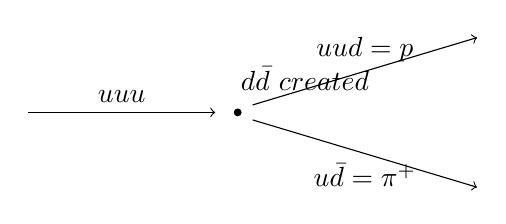
\begin{tikzpicture}[scale=0.95]
\draw[->] (-3,0) -- (-0.5,0) node[midway,above] {$uuu$};
\fill (-0.2,0) circle (1.5pt);
\draw[->] (0,0.1) -- (3,1.0) node[midway,above] {$uud=p$};
\draw[->] (0,-0.1) -- (3,-1.0) node[midway,below] {$u\bar d=\pi^+$};
\node at (0.7,0.45) {$d\bar d\ \text{created}$};
\end{tikzpicture}
\caption{Réorganisation des constituants dans la désintégration \(\Delta^{++}\rightarrow p+\pi^+\).}
\end{figure}

La conservation de la charge est immédiate :
\begin{equation}
Q(p)+Q(\pi^+)=1+1=2=Q(\Delta^{++}).
\end{equation}
Le bilan approximatif des masses permet également cette désintégration :
\begin{equation}
1200\,\mathrm{MeV}
>
940\,\mathrm{MeV}+140\,\mathrm{MeV}.
\end{equation}
Il reste suffisamment d’énergie pour que l’état final possède de l’énergie cinétique.

Les quatre particules Delta peuvent se désintégrer en un proton ou un neutron accompagné d’un pion. Leur durée de vie est extrêmement courte. On peut en estimer l’ordre de grandeur par le temps que met la lumière à traverser un proton :
\begin{equation}
\tau_\Delta
\sim
\frac{10^{-13}\,\mathrm{cm}}
     {10^{10}\,\mathrm{cm/s}}
\sim10^{-23}\,\mathrm{s}.
\end{equation}
Elles vivent néanmoins assez longtemps pour être identifiées comme des objets distincts produits dans des collisions de particules.

\begin{classroomqa}
\audiencequestion{L’ordre dans lequel les symboles \(u\) et \(d\) sont écrits a-t-il de l’importance dans ce décompte des constituants ?\lecturetimestamp{00:48:49}}
\lecturerresponse{Pas pour ce qui nous occupe. L’information importante est la composition en saveurs et la façon dont l’état quantique complet est combiné.}
\end{classroomqa}

\section{L’énigme de Pauli et la nécessité de la couleur}

La particule \(\Delta^{++}\) met au jour une contradiction. Elle est constituée de trois quarks up. Dans un état de spin \(\tfrac32\), leurs spins ordinaires peuvent tous être orientés dans la même direction. Leurs isospins sont aussi identiques, puisqu’ils sont tous \(u\). Si le spin, la saveur et l’état spatial de plus basse énergie constituaient toute la description, les trois quarks seraient des fermions identiques occupant le même état. Le principe d’exclusion de Pauli l’interdit.

\begin{classroomqa}
\audiencequestion{Comment les quarks up répétés peuvent-ils être des fermions s’ils semblent occuper le même état ?\lecturetimestamp{00:48:58}}
\lecturerresponse{Ils ne peuvent pas être identiques pour tous les nombres quantiques. La particule \(\Delta^{++}\) montre qu’il faut aux quarks une étiquette supplémentaire, au-delà du spin ordinaire, de la saveur et de l’état spatial. Cette étiquette supplémentaire est la couleur.}
\end{classroomqa}

Cette nouvelle étiquette peut prendre trois valeurs :
\begin{equation}
r,\qquad g,\qquad b,
\end{equation}
appelées rouge, vert et bleu. Ces termes n’ont aucun rapport avec la couleur visible. Ce sont des noms arbitraires désignant trois états internes. D’autres noms auraient pu être choisis ; ce qui compte, c’est qu’il existe trois possibilités distinctes.

Les versions rouge, verte et bleue d’un quark donné ont la même masse et les mêmes propriétés observables ordinaires. Elles constituent néanmoins des états quantiques distincts. Un \(\Delta^{++}\) peut donc contenir un \(u\) rouge, un \(u\) vert et un \(u\) bleu ; les trois fermions n’occupent alors pas le même état complet.

Les six saveurs sont
\begin{equation}
u,\ d,\ c,\ s,\ t,\ b.
\end{equation}
Cet ordre ne suit pas les masses. Le quark up est le plus léger, suivi du quark down. Le quark charm est beaucoup plus lourd que le quark strange, et le quark top est immensément plus lourd que le quark bottom. Chaque saveur existe dans trois couleurs. Un quark porte donc au moins deux étiquettes internes distinctes :
\begin{equation}
\text{flavor}\quad\text{and}\quad\text{color}.
\end{equation}

Les trois quarks auraient-ils pu être distingués par leur position ou leur quantité de mouvement ? L’énigme de la particule Delta concerne l’état de plus basse énergie, dont la structure spatiale et la quantité de mouvement ne peuvent fournir trois étiquettes distinctes sans modifier l’énergie et les propriétés de symétrie. La distinction manquante doit correspondre à un nouveau degré de liberté interne.

Le rôle du spin en physique atomique fournit une analogie instructive. Deux électrons qui semblent occuper le même état orbital peuvent néanmoins différer par leur état de spin. De même, des quarks identiques par leur saveur, leur spin ordinaire et leur état spatial peuvent différer par leur couleur.

\editorialnote{Le chemin historique précis faisant intervenir la spectroscopie de l’hélium, le principe de Pauli et Uhlenbeck et Goudsmit a été explicitement considéré comme incertain. L’analogie est conservée sans affirmer qu’elle correspond à la chronologie exacte de la découverte du spin.}

Yoichiro Nambu est associé à la reconnaissance du besoin de ce degré de liberté supplémentaire pour les quarks. Le point physique ne dépend pas de son nom : les trois couleurs des quarks résolvent la contradiction de Pauli. Le principe d’exclusion pertinent est le principe de Pauli, et non le principe d’incertitude de Heisenberg.

\editorialnote{L’attribution précise et l’histoire ultérieure du nom \emph{couleur} ont été laissées incertaines ; aucune chronologie plus précise n’est donc avancée ici. La mention orale du principe d’incertitude de Heisenberg est corrigée en principe d’exclusion de Pauli, conformément à l’argument sur les statistiques des fermions qui l’entoure.}

La même construction de couleur s’applique au proton et au neutron. On ne construit pas leurs états en attribuant une couleur identifiable de façon permanente à chaque symbole de saveur écrit. Un baryon physique est une superposition quantique des différentes attributions possibles du rouge, du vert et du bleu, combinées selon les symétries d’échange appropriées.

\begin{classroomqa}
\audiencequestion{La couleur est-elle une propriété physique ordinaire que l’on peut mesurer directement ?\lecturetimestamp{00:56:55}}
\lecturerresponse{Les trois couleurs ont la même masse et les mêmes propriétés ordinaires. Leur distinction se révèle de façon relationnelle, par les combinaisons permises et les processus de collision. Les expériences montrent la présence de trois états de couleur distincts, même si l’on ne peut pas préparer un quark coloré isolé pour l’examiner directement.}
\end{classroomqa}

\begin{classroomqa}
\audiencequestion{La couleur est-elle conservée ?\lecturetimestamp{00:57:38}}
\lecturerresponse{Oui. La couleur est conservée, mais les particules observables dont nous parlons ont toujours une couleur nulle ; cette loi de conservation a donc un aspect quelque peu inhabituel.}
\end{classroomqa}

\editorialnote{Plus précisément, les hadrons asymptotiques sont des singulets de couleur. L’expression ``couleur nulle'' ne désigne pas une charge abélienne nette obtenue en additionnant numériquement le rouge, le vert et le bleu.}

\begin{classroomqa}
\audiencequestion{Le proton \(uud\), à lui seul, a-t-il vraiment besoin des trois couleurs ? Il semble suffire de distinguer les deux quarks \(u\).\lecturetimestamp{00:57:58}}
\lecturerresponse{Cet exemple exige visiblement une certaine distinction supplémentaire, mais il ne rend pas le nombre trois indispensable. La particule \(\Delta^{++}\), avec ses trois quarks up de spin ordinaire parallèle et d’isospin parallèle, montre sans ambiguïté la nécessité de trois étiquettes distinctes.}
\end{classroomqa}

Voilà pourquoi les particules Delta ont joué un rôle si important. Les symétries de spin et de saveur du proton et du neutron sont plus complexes, et les détails de leurs fonctions d’onde peuvent masquer la contradiction. Pour la particule \(\Delta^{++}\), le conflit est immédiat :
\begin{equation}
uuu,\qquad
\uparrow\uparrow\uparrow,
\qquad
\text{one lowest spatial state}.
\end{equation}
Une nouvelle étiquette à trois valeurs est nécessaire. L’existence de trois états de couleur est aussi confirmée indépendamment par les données de collisions de hadrons.

Une étiquette de symétrie peut avoir un sens même lorsque ses différentes possibilités sont équivalentes prises isolément. En l’absence d’un axe spatial choisi, deux directions de spin sont physiquement équivalentes. Un second objet peut fournir un axe de référence et révéler leur relation. De même, un proton ou un neutron définit une direction dans l’espace de l’isospin, et des comparaisons avec d’autres états révèlent si les orientations internes sont parallèles ou antiparallèles. La couleur est plus subtile, mais son contenu physique se manifeste lui aussi par des relations, des corrélations et des règles d’interaction, plutôt que par une coloration visible.

On pourrait plutôt envisager d’abandonner le principe de Pauli. Il faudrait alors un nouveau cadre mathématique : la théorie quantique des champs ordinaire classe les particules comme fermions ou bosons et ne fournit aucune troisième possibilité établie qui résolve ce problème. La chromodynamique quantique conserve le caractère fermionique des quarks et introduit la couleur.

\begin{classroomqa}
\audiencequestion{Quelle observable correspond à la distinction cachée requise par le principe de Pauli ?\lecturetimestamp{01:01:08}}
\lecturerresponse{Cette question est bien plus subtile que celles des observables familières de position, de quantité de mouvement ou d’isospin. Une réponse complète nécessite d’en savoir davantage sur la dynamique de la couleur et sera donnée plus tard.}
\end{classroomqa}

\begin{classroomqa}
\audiencequestion{Le caractère fermionique des quarks a-t-il été déduit des attributions de spin des hadrons ?\lecturetimestamp{01:01:43}}
\lecturerresponse{Oui.}
\end{classroomqa}

\editorialnote{La formulation des deux questions du public précédentes est en partie indistincte. Leur sujet et les brèves réponses sont certains, mais nous n’en déduisons pas de formulation plus détaillée.}

\begin{classroomqa}
\audiencequestion{Comment associer une couleur particulière à un quark dans un proton ?\lecturetimestamp{01:01:55}}
\lecturerresponse{On n’attribue pas une couleur fixe à un constituant identifiable de façon permanente. Le proton est une superposition quantique de toutes les attributions possibles du rouge, du vert et du bleu, les facteurs de spin, de saveur, d’espace et de couleur étant symétrisés ou antisymétrisés de manière appropriée. La particule \(\Delta^{++}\) est utile parce que ses structures de spin et de saveur parallèles font apparaître la nécessité de la couleur sans qu’il soit nécessaire de connaître la fonction d’onde complète du proton.}
\end{classroomqa}

La couleur joue en chromodynamique quantique le même rôle que la charge électrique en électrodynamique : c’est le nombre quantique qui régit l’interaction. La chromodynamique quantique rend compte avec une grande précision des données expérimentales issues des collisions de hadrons. La justification ultime de ce cadre théorique tient à l’accord de ses conséquences avec l’expérience.

\section{Photons et gluons}

Les quarks sont les particules de matière fermioniques de la QCD, analogues aux électrons en QED sous ce rapport limité. Qu’est-ce qui les lie ?

En électrodynamique, un électron est une source de champ électromagnétique. Dans le langage des particules, il émet et absorbe des photons, et l’échange de photons produit des forces entre particules chargées. De même, un quark est une source du champ de gluons et peut émettre et absorber des gluons.

Les gluons ressemblent aux photons à plusieurs égards importants. Ce sont des particules sans masse de spin 1, qui possèdent des états de polarisation analogues à ceux des photons. Leur quantité de mouvement et leur polarisation sont des propriétés dynamiques ordinaires. La différence essentielle est que les gluons portent une information de couleur et interagissent donc entre eux.

Les photons ne portent pas de charge électrique. Au niveau élémentaire de la QED, un photon n’en émet pas un autre, et deux faisceaux lumineux se traversent sans interagir. Il existe de très faibles interactions photon-photon d’ordre supérieur faisant intervenir des boucles d’électrons, mais ce sont des effets secondaires, et non un couplage direct d’un photon à lui-même. Dans le vide, le vertex élémentaire de la QED se réduit simplement à un électron qui émet ou absorbe un photon.

\begin{figure}[h]
\centering
\begin{tikzpicture}[scale=1.0]
\draw[->] (-2,-1) -- (0,0);
\draw[->] (0,0) -- (2,-1);
\draw[smooth] plot coordinates {
(0,0) (0.16,0.27) (0.32,0.23) (0.48,0.52)
(0.64,0.48) (0.80,0.77) (0.96,0.73)
(1.12,1.02) (1.28,0.98) (1.44,1.27)
(1.60,1.23) (1.76,1.52)
};
\node at (-1.25,-0.75) {$e^-$};
\node at (1.25,-0.75) {$e^-$};
\node at (1.95,1.62) {$\gamma$};
\fill (0,0) circle (1.5pt);
\end{tikzpicture}
\caption{Vertex élémentaire de la QED : un électron émet ou absorbe un photon.}
\end{figure}

Inverser le sens d’une ligne fermionique transforme l’interprétation en électron en une interprétation en positron. L’émission, l’absorption et les processus croisés avec un positron sont autant de réarrangements de ce même vertex.

Pour les besoins du calcul, on peut faire comme si un photon possédait certaines propriétés d’une paire électron--positron. Cette paire est électriquement neutre, et les spins alignés de l’électron et du positron peuvent donner un spin total égal à 1. Si une interaction externe fournit l’énergie et la quantité de mouvement nécessaires, un photon peut produire une paire électron--positron. Cela ne signifie en rien qu’un photon soit littéralement constitué d’un électron et d’un positron. L’image de la paire fictive apporte peu à la QED elle-même, mais son analogue en couleur est utile en QCD.

\section{Étiquettes de couleur--et d’anticouleur des gluons}

Représentons les trois états de couleur d’un quark par une colonne :
\begin{equation}
q=
\begin{pmatrix}
r\\
g\\
b
\end{pmatrix}.
\end{equation}
Représentons les étiquettes correspondantes des antiquarks par une ligne :
\begin{equation}
\bar q=
\begin{pmatrix}
\bar r&\bar g&\bar b
\end{pmatrix}.
\end{equation}

Un gluon n’est pas un état lié quark--antiquark. Toutefois, son étiquetage en couleur se comporte comme s’il portait une couleur et une anticouleur. On peut donc organiser les étiquettes possibles ainsi :
\begin{equation}
\begin{pmatrix}
r\bar r&r\bar g&r\bar b\\
g\bar r&g\bar g&g\bar b\\
b\bar r&b\bar g&b\bar b
\end{pmatrix}.
\end{equation}
À première vue, cela donne neuf combinaisons.

\begin{classroomqa}
\audiencequestion{Les entrées diagonales couleur--anticouleur sont-elles indiscernables ?\lecturetimestamp{01:13:37}}
\lecturerresponse{Pas exactement. Les entrées diagonales sont distinctes ; le point est que leur somme ne constitue pas un état quantique indépendant.}
\end{classroomqa}

En réalité, il n’existe que huit états indépendants de gluon. Les trois étiquettes diagonales ne sont pas simplement indiscernables les unes des autres, mais la somme diagonale particulière
\begin{equation}
r\bar r+g\bar g+b\bar b
\end{equation}
ne fournit pas de gluon supplémentaire indépendant en QCD. L’explication plus profonde de cette réduction sera donnée plus tard. Pour les raisonnements actuels sur les flux de couleur, il est utile de travailler avec les neuf étiquettes apparentes, en gardant à l’esprit qu’une combinaison diagonale est absente.

\section{Le vertex quark--gluon}

Un quark peut émettre un gluon et ressortir avec la même couleur ou une couleur différente. Si un quark entre avec la couleur \(a\) et ressort avec la couleur \(b\), le gluon émis porte l’étiquette de calcul \(a\bar b\) :
\begin{equation}
a\longrightarrow b+(a\bar b).
\end{equation}
Par exemple,
\begin{equation}
r\longrightarrow g+(r\bar g).
\end{equation}
La ligne de couleur rouge se prolonge dans le gluon, tandis que la ligne verte se prolonge à travers le quark sortant et s’inverse en une ligne antig verte dans le gluon.

Le quark n’est pas obligé de changer de couleur. La même règle permet aussi :
\begin{equation}
r\longrightarrow r+(r\bar r),
\end{equation}
ou
\begin{equation}
r\longrightarrow b+(r\bar b).
\end{equation}

\begin{figure}[h]
\centering
\begin{tikzpicture}[scale=1.0]
\draw[->] (-2,-0.8) -- (0,0) node[midway,above] {$r$};
\draw[->] (0,0) -- (2,0.9) node[midway,above] {$g$};
\draw[smooth] plot coordinates {
(0,0) (0.20,-0.23) (0.40,-0.17) (0.60,-0.46)
(0.80,-0.40) (1.00,-0.69) (1.20,-0.63)
(1.40,-0.92) (1.60,-0.86) (1.80,-1.15)
(2.00,-1.09)
};
\node at (2.35,-1.12) {$r\bar g$};
\fill (0,0) circle (1.5pt);
\end{tikzpicture}
\caption{Un quark rouge devient vert en émettant un gluon \(r\bar g\).}
\end{figure}

C’est l’un des éléments constitutifs élémentaires de la QCD.

\begin{classroomqa}
\audiencequestion{Un gluon ne peut-il être émis que si le quark change de couleur ?\lecturetimestamp{01:17:15}}
\lecturerresponse{Non. Le quark sortant peut avoir la même couleur ou une couleur différente. Dans les deux cas, l’étiquette couleur--anticouleur du gluon assure la continuité des lignes de couleur.}
\end{classroomqa}

\section{Le vertex à trois gluons}

La QCD possède une autre interaction élémentaire sans analogue élémentaire en QED : un gluon peut interagir directement avec d’autres gluons.

Partons d’un gluon \(r\bar b\). Dans le langage des flux de couleur, il peut se séparer ainsi :
\begin{equation}
r\bar b
\longrightarrow
r\bar g+g\bar b.
\end{equation}
La ligne rouge se prolonge dans \(r\bar g\), la ligne antibleue se prolonge dans \(g\bar b\), et la paire vert-antivert relie les deux gluons sortants. On obtient ainsi un vertex à trois gluons.

\begin{figure}[h]
\centering
\begin{tikzpicture}[scale=1.0]
\draw[smooth] plot coordinates {
(-2,0) (-1.80,0.12) (-1.60,-0.02) (-1.40,0.12)
(-1.20,-0.02) (-1.00,0.12) (-0.80,-0.02)
(-0.60,0.12) (-0.40,-0.02) (-0.20,0.12) (0,0)
};
\draw[smooth] plot coordinates {
(0,0) (0.20,0.27) (0.40,0.21) (0.60,0.50)
(0.80,0.44) (1.00,0.73) (1.20,0.67)
(1.40,0.96) (1.60,0.90) (1.80,1.19) (2.00,1.13)
};
\draw[smooth] plot coordinates {
(0,0) (0.20,-0.27) (0.40,-0.21) (0.60,-0.50)
(0.80,-0.44) (1.00,-0.73) (1.20,-0.67)
(1.40,-0.96) (1.60,-0.90) (1.80,-1.19) (2.00,-1.13)
};
\node at (-2.45,0) {$r\bar b$};
\node at (2.45,1.18) {$r\bar g$};
\node at (2.45,-1.18) {$g\bar b$};
\fill (0,0) circle (1.5pt);
\end{tikzpicture}
\caption{Flux de couleur au vertex à trois gluons : \(r\bar b\rightarrow r\bar g+g\bar b\).}
\end{figure}

Il n’est pas nécessaire de mémoriser toutes les combinaisons possibles. Suivez chaque ligne de couleur dans le diagramme. Lorsqu’une ligne fermionique inverse son sens temporel, réinterprétez-la comme la ligne de l’antiparticule ou de l’anticouleur correspondante.

\section{Échange de gluons et forces}

Un gluon produit des forces par échange, tout comme un photon produit des forces électromagnétiques lorsqu’il est échangé entre des particules chargées.

Par exemple, un quark bleu et un antiquark antib leu peuvent échanger un gluon \(g\bar b\) et ressortir sous forme d’un quark vert et d’un antiquark antig vert. Une attribution des flux de couleur compatible avec les deux vertex est \footnote{La variation nette de couleur \(b+\bar b\longrightarrow g+\bar g\) est explicite, mais les étiquettes locales de couleur sont corrigées à plusieurs reprises. L’étiquette échangée \(g\bar b\) se déduit en imposant la continuité des flux de couleur aux deux vertex.}
\begin{equation}
b+\bar b
\longrightarrow
g+\bar g.
\end{equation}
Au vertex de l’antiquark,
\begin{equation}
\bar b\longrightarrow\bar g+(g\bar b),
\end{equation}
tandis qu’au vertex du quark,
\begin{equation}
b+(g\bar b)\longrightarrow g.
\end{equation}
Le gluon échangé transporte le changement de couleur d’une ligne fermionique à l’autre.

\begin{figure}[h]
\centering
\begin{tikzpicture}[scale=1.0]
\draw[->] (-1.8,0) -- (-1.8,-1.8) node[midway,left] {$\bar b$};
\draw[->] (-1.8,1.8) -- (-1.8,0) node[midway,left] {$\bar g$};
\draw[->] (1.8,-1.8) -- (1.8,0) node[midway,right] {$b$};
\draw[->] (1.8,0) -- (1.8,1.8) node[midway,right] {$g$};
\draw[smooth] plot coordinates {
(-1.8,0) (-1.50,0.13) (-1.20,-0.03) (-0.90,0.13)
(-0.60,-0.03) (-0.30,0.13) (0,-0.03)
(0.30,0.13) (0.60,-0.03) (0.90,0.13)
(1.20,-0.03) (1.50,0.13) (1.8,0)
};
\node at (0,0.42) {$g\bar b$};
\fill (-1.8,0) circle (1.5pt);
\fill (1.8,0) circle (1.5pt);
\end{tikzpicture}
\caption{L’échange d’un gluon \(g\bar b\) transforme une paire quark bleu--antiquark antib leu en une paire quark vert--antiquark antig vert ; les flèches des antiquarks pointent dans le sens opposé au temps croissant.}
\end{figure}

La même interaction permet des forces entre gluons. Une réalisation cohérente est \footnote{Le cours établit l’échange de gluons entre gluons et la règle consistant à suivre les lignes, mais les étiquettes locales du diagramme sont révisées à plusieurs reprises. L’attribution représentée est une réalisation cohérente de la règle finale, et non une transcription certaine de chacune des étiquettes intermédiaires.}
\begin{equation}
(r\bar b)+(b\bar r)
\longrightarrow
(r\bar g)+(g\bar r),
\end{equation}
avec un gluon \(g\bar b\) échangé entre les deux gluons externes :
\begin{align}
r\bar b&\longrightarrow r\bar g+g\bar b,\\
b\bar r+g\bar b&\longrightarrow g\bar r.
\end{align}

\begin{figure}[h]
\centering
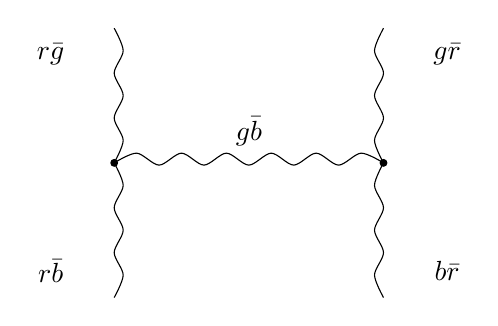
\begin{tikzpicture}[scale=0.95]
\draw[smooth] plot coordinates {
(-1.8,-1.8) (-1.68,-1.50) (-1.80,-1.20) (-1.68,-0.90)
(-1.80,-0.60) (-1.68,-0.30) (-1.8,0)
};
\draw[smooth] plot coordinates {
(-1.8,0) (-1.68,0.30) (-1.80,0.60) (-1.68,0.90)
(-1.80,1.20) (-1.68,1.50) (-1.8,1.8)
};
\draw[smooth] plot coordinates {
(1.8,-1.8) (1.68,-1.50) (1.80,-1.20) (1.68,-0.90)
(1.80,-0.60) (1.68,-0.30) (1.8,0)
};
\draw[smooth] plot coordinates {
(1.8,0) (1.68,0.30) (1.80,0.60) (1.68,0.90)
(1.80,1.20) (1.68,1.50) (1.8,1.8)
};
\draw[smooth] plot coordinates {
(-1.8,0) (-1.50,0.13) (-1.20,-0.03) (-0.90,0.13)
(-0.60,-0.03) (-0.30,0.13) (0,-0.03)
(0.30,0.13) (0.60,-0.03) (0.90,0.13)
(1.20,-0.03) (1.50,0.13) (1.8,0)
};
\node at (-2.65,-1.45) {$r\bar b$};
\node at (-2.65,1.45) {$r\bar g$};
\node at (2.65,-1.45) {$b\bar r$};
\node at (2.65,1.45) {$g\bar r$};
\node at (0,0.42) {$g\bar b$};
\fill (-1.8,0) circle (1.5pt);
\fill (1.8,0) circle (1.5pt);
\end{tikzpicture}
\caption{Échange d’un gluon \(g\bar b\) entre deux gluons, chaque ligne de couleur et d’anticouleur se prolongeant à travers les vertex.}
\end{figure}

\section{Auto-interaction des gluons et champs non linéaires}

L’auto-interaction des gluons change la nature de la QCD. Les quarks peuvent se lier par échange de gluons et former des hadrons, mais les gluons peuvent aussi se lier entre eux par échange de gluons. La QCD peut donc contenir des objets composites entièrement constitués de degrés de liberté gluoniques, sans quarks. En QED, il n’existe pas d’état lié élémentaire correspondant qui soit composé uniquement de photons.

Le langage des champs mène à la même conclusion. Dans le vide, deux ondes électromagnétiques se traversent sans interagir au niveau élémentaire. Deux ondes de gluons interagissent et se déforment mutuellement. Même différentes parties d’une seule configuration du champ de gluons peuvent exercer des forces les unes sur les autres. Le champ de gluons est donc non linéaire.

\begin{classroomqa}
\audiencequestion{Doit-on trouver le même nombre d’étiquettes rouges, vertes et bleues de chaque côté d’un diagramme ?\lecturetimestamp{01:24:59}}
\lecturerresponse{La règle pratique consiste à suivre chaque ligne de couleur dans le diagramme. Cette continuité exprime la conservation de la couleur. Si une ligne fermionique fait demi-tour dans le temps, son étiquette devient celle de l’antiparticule ou de l’anticouleur correspondante.}
\end{classroomqa}

\begin{classroomqa}
\audiencequestion{Toutes les étiquettes de couleur et d’anticouleur de la première version du diagramme sont-elles cohérentes ?\lecturetimestamp{01:26:00}}
\lecturerresponse{Non. Plusieurs étiquettes doivent être corrigées. Dans une attribution cohérente, les lignes rouge, antibleue et verte se prolongent chacune à travers les vertex ; une flèche fermionique inversée s’interprète comme celle d’une antiparticule.}
\end{classroomqa}

\begin{classroomqa}
\audiencequestion{Traite-t-on une ligne de gluon intermédiaire comme une paire quark--antiquark ?\lecturetimestamp{01:27:58}}
\lecturerresponse{Uniquement pour l’étiquetage de couleur. Un gluon n’est pas littéralement un composite quark--antiquark, mais il porte les propriétés de couleur et d’anticouleur correspondantes.}
\end{classroomqa}

À ce stade, les règles élémentaires sont concises :

\begin{itemize}
\item les quarks émettent et absorbent des gluons ;
\item les gluons interagissent directement avec d’autres gluons ;
\item chaque ligne de couleur et d’anticouleur doit se prolonger à travers un vertex ;
\item l’inversion temporelle d’une ligne fermionique la transforme en la ligne de l’antiparticule correspondante.
\end{itemize}

\begin{classroomqa}
\audiencequestion{Les gluons restent-ils sans masse lorsqu’on les représente par toutes ces lignes de couleur--anticouleur ?\lecturetimestamp{01:28:13}}
\lecturerresponse{Oui. Les gluons restent sans masse. La précision qui suit concerne le sens de la masse attribuée à un quark à l’intérieur d’un hadron.}
\end{classroomqa}

Nous allons maintenant aborder le confinement et la structure des hadrons : pourquoi on n’observe jamais de couleur isolée et comment quarks et gluons s’organisent à l’intérieur de particules composites. Il est d’abord utile de préciser ce que l’on entend par masse d’un quark constituant.

\section{Échelle de sondage et sens de la masse du quark}

Imaginons un petit objet de masse \(m\) fixé à un morceau de matériau souple et déformable---, par exemple un morceau de chewing-gum qui pend. Appliquons une force très faible, assez lentement pour que le matériau souple ait le temps de s’adapter et que tout le système se déplace ensemble. L’inertie mesurée est alors celle du petit objet plus celle du matériau qui lui est fixé.

Faisons maintenant osciller le petit objet à très haute fréquence. Le matériau souple n’a pas le temps de suivre le mouvement rapide. Il reste presque immobile tandis que le petit cœur réagit. L’inertie mesurée à haute fréquence est alors beaucoup plus proche de celle de \(m\) seul.

\begin{figure}[h]
\centering
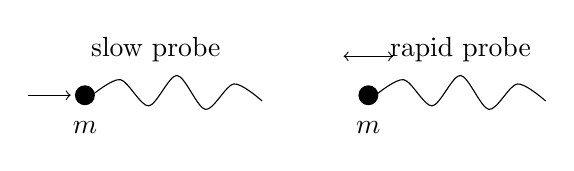
\begin{tikzpicture}[scale=0.9]
\fill (-3,0) circle (4pt);
\node at (-3,-0.45) {$m$};
\draw[smooth] plot coordinates {
(-2.9,0) (-2.5,0.22) (-2.1,-0.15) (-1.7,0.28)
(-1.3,-0.20) (-0.9,0.16) (-0.5,-0.08)
};
\draw[->] (-3.8,0) -- (-3.2,0);
\node at (-2.0,0.65) {slow probe};

\fill (1.0,0) circle (4pt);
\node at (1.0,-0.45) {$m$};
\draw[smooth] plot coordinates {
(1.1,0) (1.5,0.22) (1.9,-0.15) (2.3,0.28)
(2.7,-0.20) (3.1,0.16) (3.5,-0.08)
};
\draw[<->] (0.65,0.55) -- (1.35,0.55);
\node at (2.3,0.65) {rapid probe};
\end{tikzpicture}
\caption{Un sondage lent met en mouvement le cœur et son attache souple ensemble, tandis qu’un sondage rapide mesure d’abord principalement la réponse du cœur.}
\end{figure}

Il s’agit d’une analogie classique. La masse inférée dépend de la fréquence de la force appliquée, car les différentes parties du système ont le temps de participer à des fréquences différentes.

Un quark à l’intérieur d’un hadron est entouré de matière gluonique en forte interaction et des autres constituants. Si l’on pouvait tirer très lentement sur un quark, le hadron entier réagirait. L’inertie rencontrée serait alors de l’ordre de la masse du nucléon,
\begin{equation}
m_N\sim930\text{--}940\,\mathrm{MeV}.
\end{equation}
Si l’on frappait le quark très fort et le sondait sur un temps très bref, la réponse initiale serait associée au paramètre de masse beaucoup plus petit conventionnellement attribué à un quark léger, soit environ
\begin{equation}
m_{u,d}\sim5\text{--}10\,\mathrm{MeV}
\end{equation}
dans les estimations utilisées ici.

L’expression ``la masse d’un quark'' exige donc de préciser l’échelle du sondage. Une perturbation douce, de basse fréquence, met en mouvement le composite étendu ; une perturbation intense, de haute fréquence, en résout d’abord une partie beaucoup plus petite. Cette analogie ne constitue pas une dérivation de la renormalisation, mais elle motive la dépendance des paramètres servant à décrire les particules envers les fréquences et les longueurs d’onde des interactions au cours desquelles on les mesure. Ces paramètres dépendant de l’échelle sont appelés paramètres courants ou constantes courantes.

\begin{classroomqa}
\audiencequestion{Cette masse dépendant de la fréquence n’est-elle qu’une reformulation d’une relation d’incertitude telle que \(\Delta x\,\Delta t\) ?\lecturetimestamp{01:33:32}}
\lecturerresponse{Non. L’exemple est déjà un phénomène classique. Sous l’action d’une force rapide, une petite masse fixée à quelque chose de souple accélère d’une certaine façon ; sous l’action d’une force lente, elle accélère autrement, car une quantité différente du matériau qui lui est fixé a le temps de réagir.}
\end{classroomqa}

\begin{classroomqa}
\audiencequestion{La discussion précédente de la charge électrique de l’électron faisait-elle intervenir le même type de dépendance à l’échelle ?\lecturetimestamp{01:34:04}}
\lecturerresponse{Oui. La leçon générale est que les paramètres servant à décrire les particules dépendent des fréquences et des longueurs d’onde des interactions auxquelles elles sont sondées. On les appelle constantes courantes.}
\end{classroomqa}

\begin{classroomqa}
\audiencequestion{La même précision s’applique-t-elle à la charge fractionnaire attribuée à un quark ?\lecturetimestamp{01:34:36}}
\lecturerresponse{Oui. Il faut définir soigneusement ce que l’on entend par charge d’un quark. À ce niveau, elle est donnée par rapport à la charge du proton ; une définition plus complète fera l’objet d’une discussion distincte.}
\end{classroomqa}

\editorialnote{Le nombre quantique fixe de charge électrique fractionnaire et le couplage d’interaction dépendant de l’échelle sont deux choses distinctes. Le caractère courant du couplage ne modifie pas les étiquettes de saveur \(+\tfrac23\) ni \(-\tfrac13\) elles-mêmes.}

\begin{classroomqa}
\audiencequestion{Pourquoi l’étiquetage de couleur fait-il toujours intervenir un quark et un antiquark ? Pourquoi deux quarks ne pourraient-ils pas former l’objet correspondant ?\lecturetimestamp{01:34:55}}
\lecturerresponse{C’est une question importante, mais sa réponse relève de la prochaine discussion sur les combinaisons de couleur permises et le confinement.}
\end{classroomqa}

\begin{classroomqa}
\audiencequestion{Si l’on ne peut pas isoler les quarks individuellement, comment la charge fractionnaire, la couleur et le modèle des quarks ont-ils été déduits ?\lecturetimestamp{01:35:17}}
\lecturerresponse{Cette représentation s’est élaborée progressivement à partir de nombreux indices, ainsi que de contradictions apparentes. Les régularités des hadrons suggéraient des constituants quark ; les états Delta ont révélé un conflit avec la statistique de Fermi ; et le confinement permanent des quarks constituait un autre fait singulier. L’hypothèse des quarks est apparue au début des années 1960, Nambu a proposé très tôt une version importante de l’idée de couleur, et de nombreux physiciens ont assemblé et mis à l’épreuve la structure complète au cours de la dizaine d’années qui a suivi. Elle ne résultait ni d’une seule observation ni du travail d’une seule personne.}
\end{classroomqa}

\begin{classroomqa}
\audiencequestion{Pourquoi n’y a-t-il que huit gluons plutôt que les neuf combinaisons couleur--anticouleur apparentes ?\lecturetimestamp{01:37:24}}
\lecturerresponse{L’explication détaillée de l’absence d’un gluon supplémentaire correspondant à la somme diagonale est reportée à plus tard.}
\end{classroomqa}

\begin{classroomqa}
\audiencequestion{Cette discussion de la QCD fait-elle abstraction des électrons ?\lecturetimestamp{01:37:33}}
\lecturerresponse{Oui. On isole ici la QCD de la même manière qu’une discussion de la QED peut provisoirement faire abstraction des quarks. Il faudra finalement réunir ces secteurs dans une structure plus vaste comprenant les quarks, les électrons, les photons et les autres particules. Une partie de cette synthèse a été réalisée, tandis qu’une autre reste inachevée. En physique, on procède souvent en isolant un sous-système, en le comprenant, puis en réassemblant les éléments.}
\end{classroomqa}